\chapter{Background} \label{ch:background}
Given that robots are becoming more prevalent in the industry, as stated in the previous chapter. It is with increasing benefit that robots can be controlled using non-experts. Several papers use Natural Language Processing (NLP) as a tool for decreasing robot control complexity. 
An approach to NLP for robot control could be to use neural networks to directly map input Natural Language (NL) to robot actions\cite{Method1}. The advantage of using this technique is that it removes the need to analyze the input deterministically, as this is a difficult task for NL. But this method also relies on unique training data that, in the given paper, had to be created manually.
Another approach is to use neural networks to map NL into a deterministic language called Robot Control Language\cite{Method2}. The neural network is trained on data pairs consisting of NL commands and their respective RCL expressions. Whereafter a processing technique relying on the syntactical analysis of Robot Control Language is used to determine the actions. Mapping to RCL is a simpler goal, than mapping directly to actions, due to the neural network performing a subtask instead of processing NL to robot motion. The advantage is the combinatory use of a neural network to process NL, and afterward, a syntactical parser to determine the actions within the RCL expression. By parting the task into two subtasks the complexity of the neural network is reduced. The disadvantage shown in the paper is that training data again was gathered manually.
The last approach uses both preprocessing and postprocessing, which is done before and after the neural network categorization process respectively\cite{Method3}. The preprocessing tool identifies possible commands before the sentence is split up into subsentences and fed through a neural network one subsentence at a time. The postprocessing stitches the actions back together before movement is executed on the robot. This paper intends to ease the neural network process load, by preprocessing the NL command before input. This is done, as it is known, that neural networks trained on self-created data, is a difficult task, due to lack of training data. 
\\\\
The general theme is to mainly use a neural network categorization tool and compensate for the workload so that the neural network task is simplified. The simplification is due to the lack of complexity of the neural network models, that in turn is caused by the limited availability of task-specific datasets.
Neural networks will also be used in this thesis. But for this thesis, neural networks are used as a linguistic language model that outputs grammatical analysis information regardless of robot context. Using grammatical analysis language models enables the use of models trained on online available datasets, that are not task-specific. Furthermore, it also allows the use of pre-trained language models made in previous studies, which significantly lowers neural network implementation time. Also, by removing the time constraint of creating neural networks, several neural networks can be implemented to further gain more grammatical information from NL inputs.
\\\\
To analyze the grammatical information, a parser is created, that uses the information to extract the robot movement actions. The actions are then executed by a robot.
\\\\
Since the thesis uses neural networks, a short explanation of the most used neural network models is given.
The following sections go into detail about how transformers work and shortly on how LSTMs work.


\section{Transformers} \label{sec:TF}

Transformers are a neural network tool for Natural Language Processing (NLP). This section focuses on the details of how transformers work.

The reason why transformers are mentioned is because of their widespread use as an NLP tool. Their popularity can be seen based on the GLUE benchmark\cite{wang2018glue}, where the leaderboard is dominated by bert models (a transformer neural network).
The transformers have multiple features, including enhanced training efficiency and constant sentence dependency path length. 

The idea of sentence dependency path length is illustrated on figure \ref{fig:path_length}, where an example of a path length between 'move' and 'point 0' is shown. Normally, the word 'point 0' would be two words having their index. But it is treated as one word in this example. The length between the two words is 9 words. Different methods have different path length complexities for finding dependencies this is illustrated in table \ref{table:path_length_complexity}. Given this table, it is observed that transformers have the smallest path length of the three types, as it is constant.


\begin{figure}[ht]
    \centering
    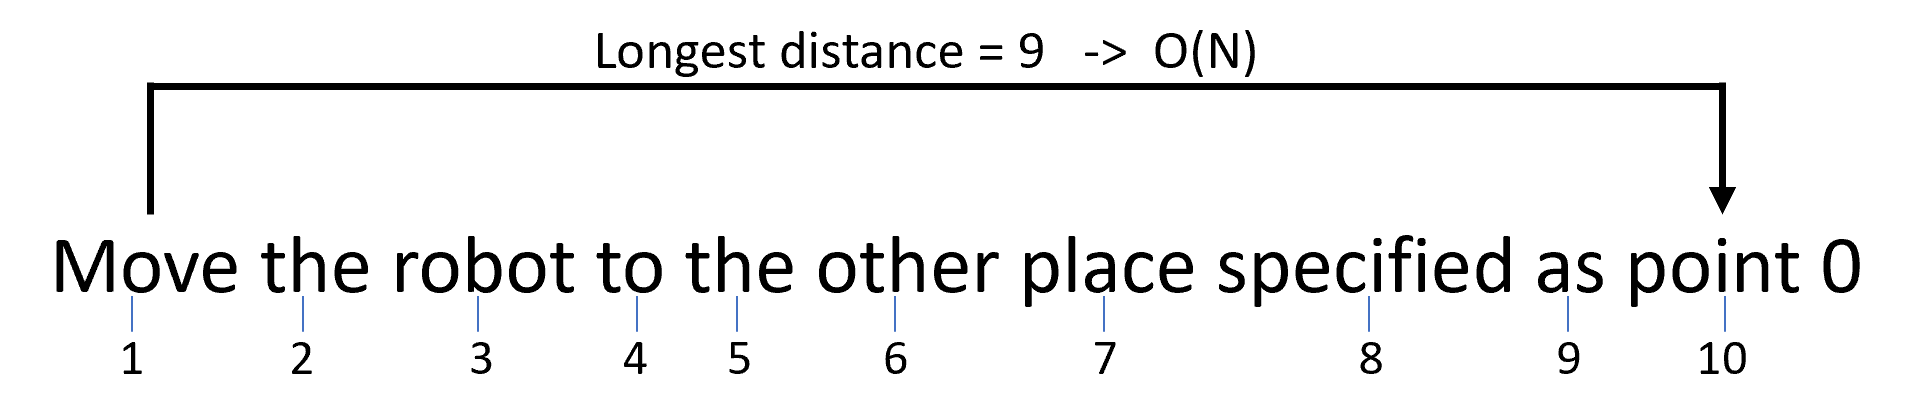
\includegraphics[width=8cm]{img/dependency_path_length.png}
    \caption{Figure shows the maximum path length between the word 'move' and the word 'point 0'.}
    \label{fig:path_length}
\end{figure}

\begin{table}[ht]
    \centering
    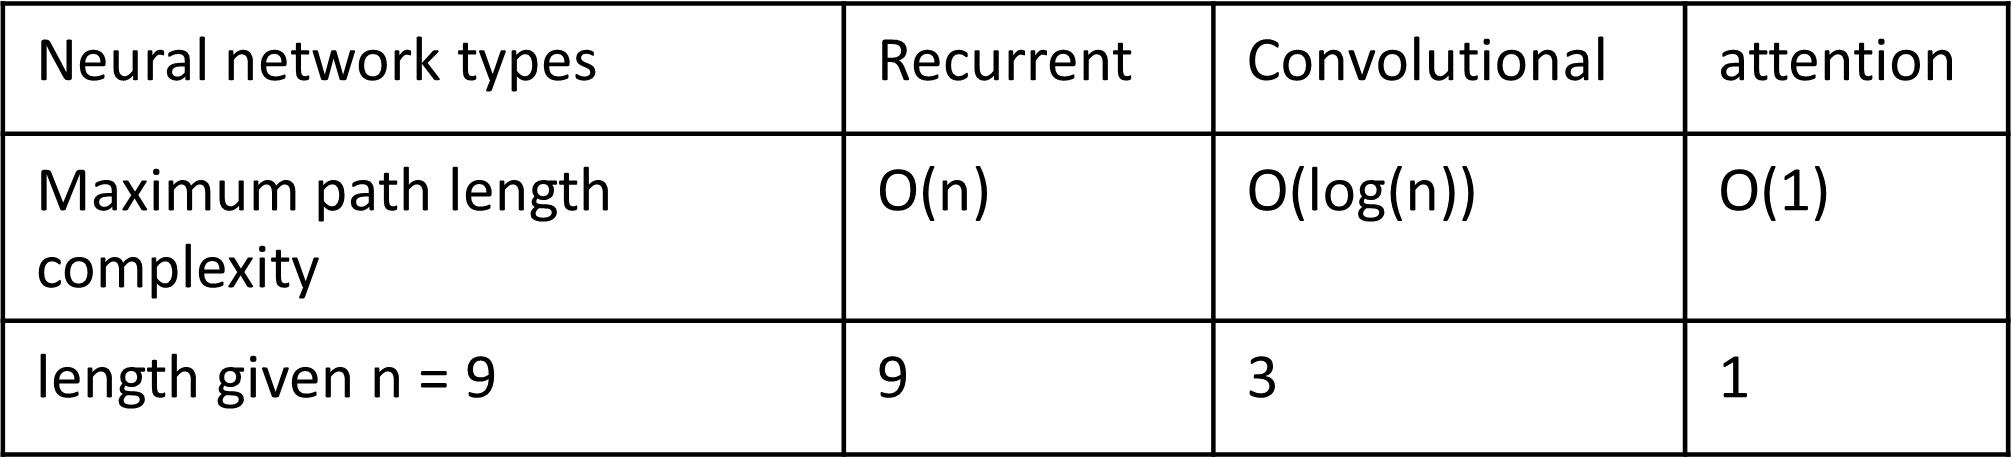
\includegraphics[width=8cm]{img/path_complexity.png}
    \caption{Table showing the maximum path length of the sentence in the previous figure.}
    \label{table:path_length_complexity}
\end{table}

Both of these features (training efficiency, and a constant dependency path length) are effects of the attention-based model design. Transformers use a neural network layer called multi-headed attention to compute every word in parallel. This both enhances parallel training potential and trivializes sentences with long dependencies, as attention heads can be used to compute the dependency path length of any sentence in constant time. The following sections go into detail about how transformers work.


\subsection{Transformer design}\label{subsec:TD}
The transformer model is as shown in figure \ref{fig:TD}. The rest of the subsections goes through the process of how the transformer works based on this figure.
 
\begin{figure}[ht]
    \centering
    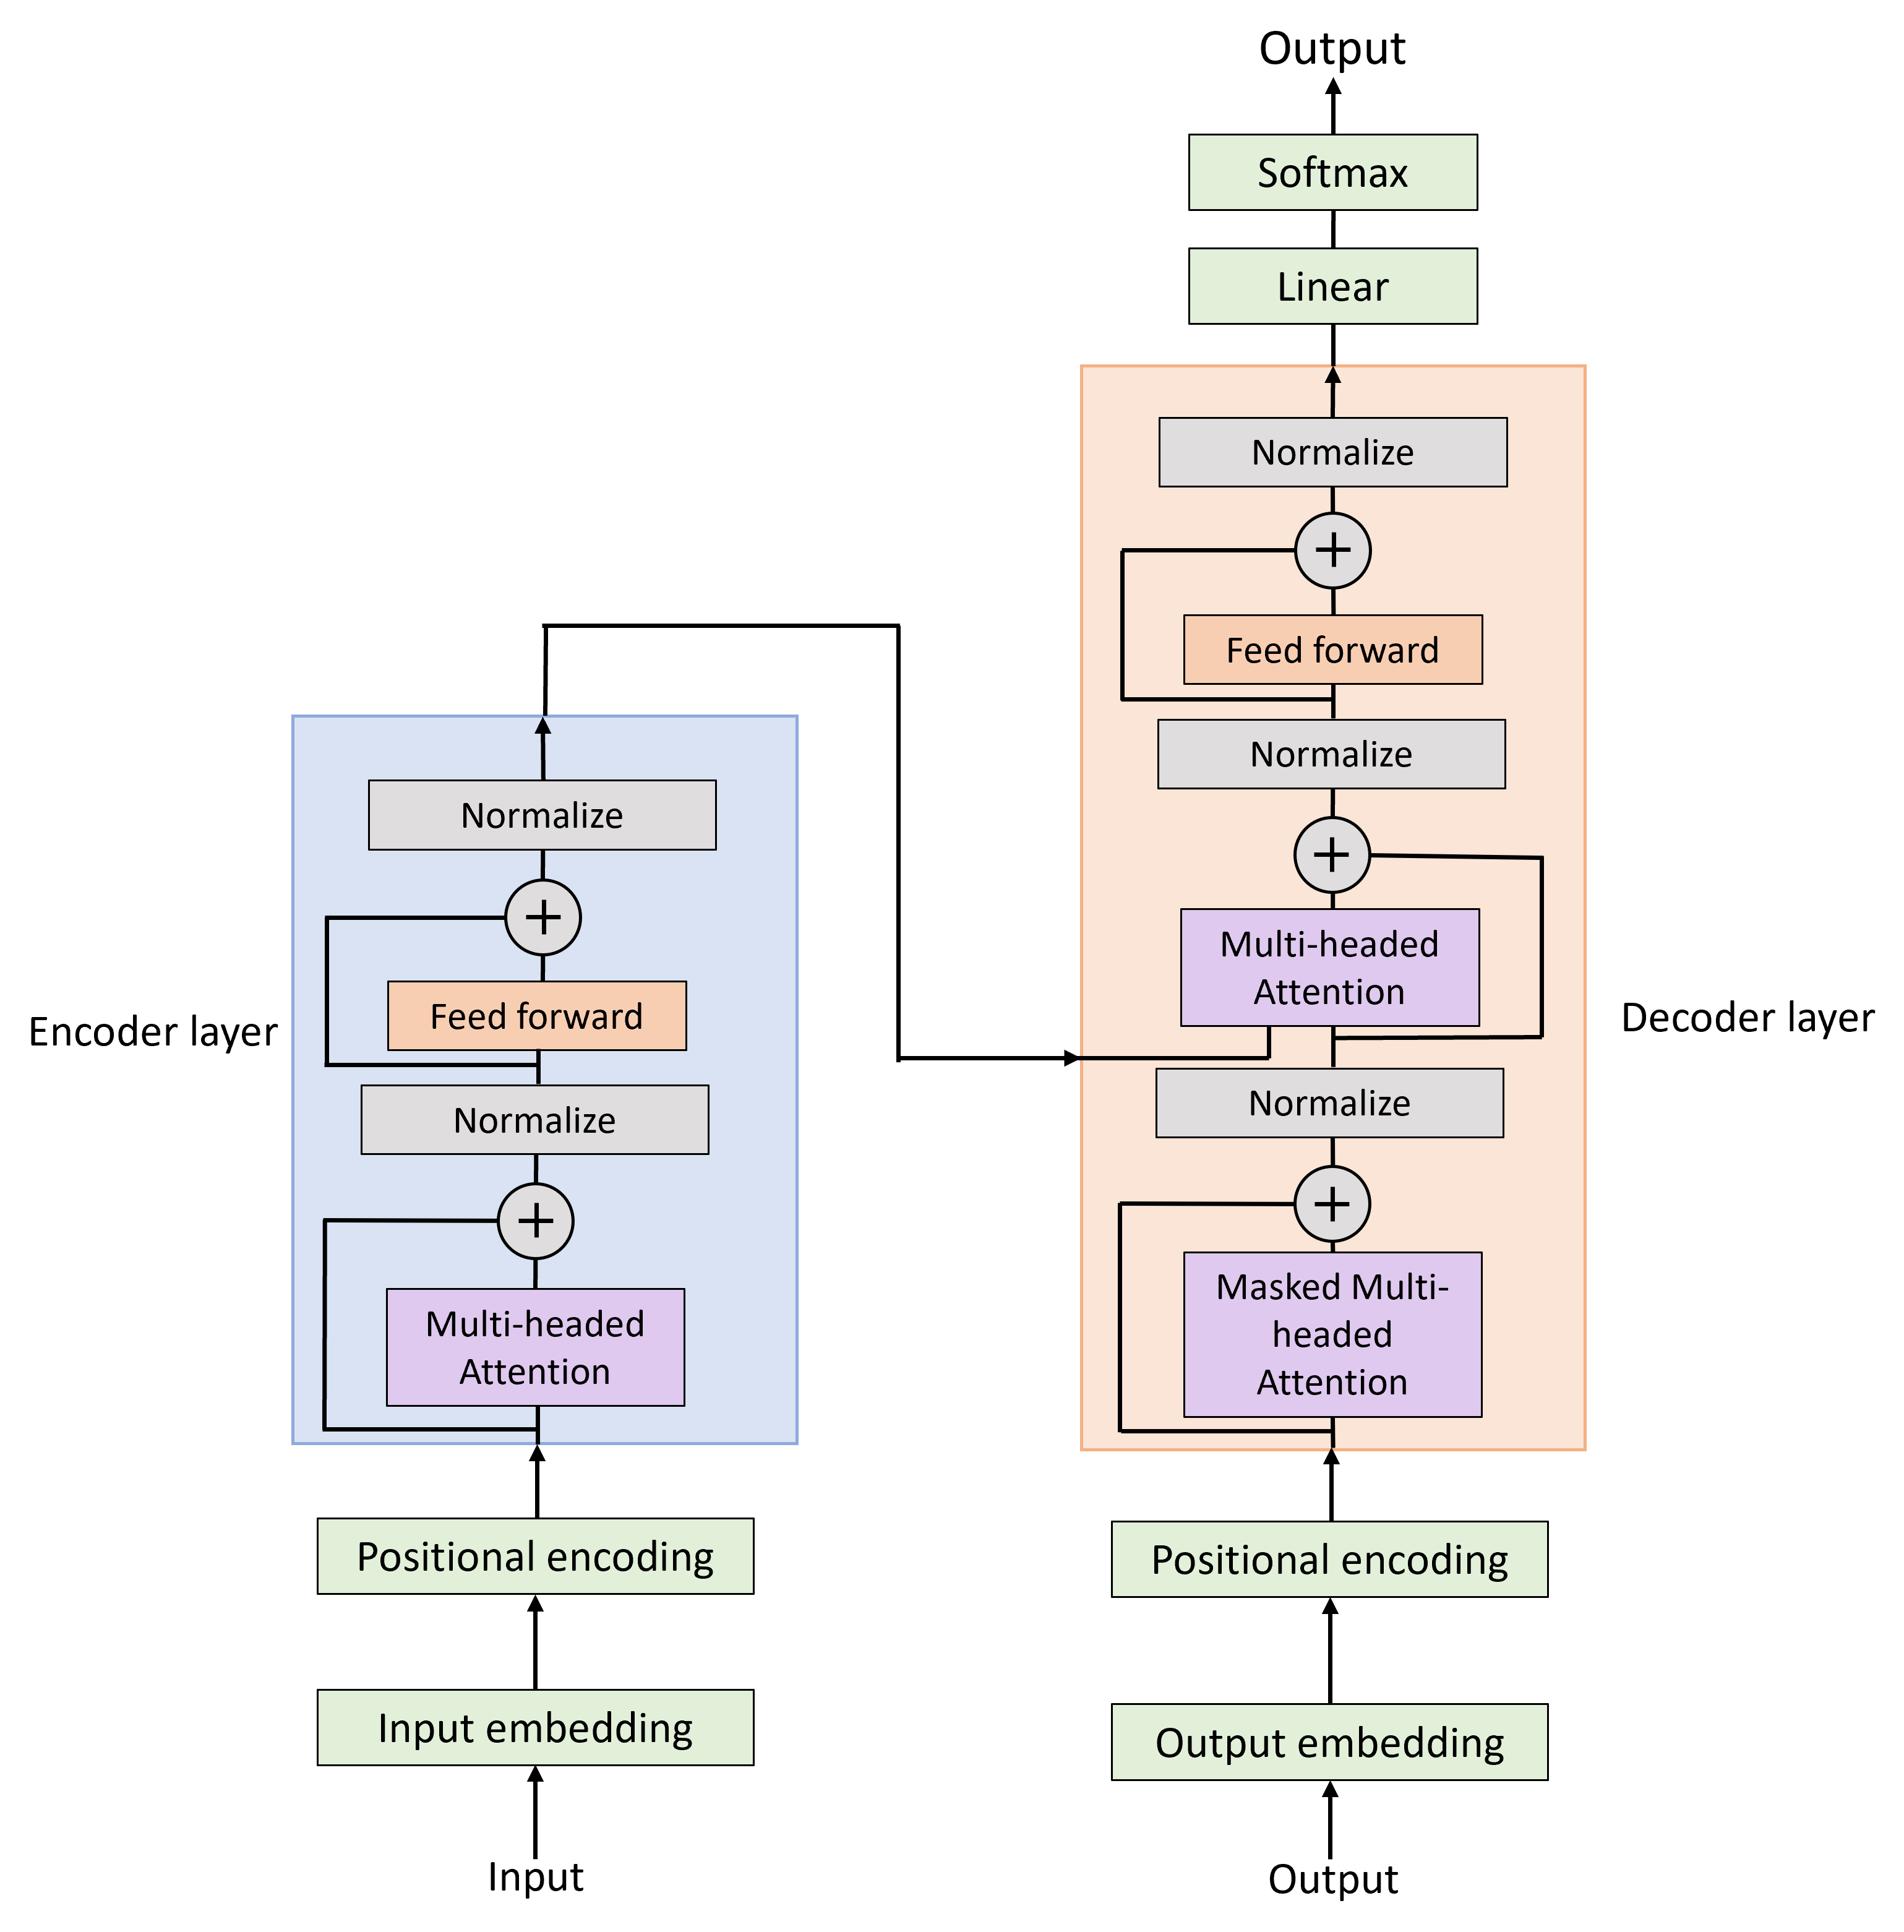
\includegraphics[width=10cm]{img/transformer_model.png}
    \caption{Figure presenting the transformer model with inspiration from \cite{46201}}
    \label{fig:TD}
\end{figure}


\subsection{Word embeddings and positional embeddings} \label{sec:WE}
The transformer input is passed into a word embedding. Word embeddings transform words into high-dimensional vector representations. It is trained separately, usually by predicting the next word in a training sentence, to capture the semantic word-to-word relation. The second transformation in the pipeline is positional embedding. Positional embedding is a transformation that injects values into the vector representations depending on the indexation of the vector. This is an essential part of the transformer pipeline, as it gives positional information to the vector transformation, that transformers would not gain otherwise. The reason is a side effect of the Transformers' constant complexity for dependency path length. 
\\\\
Afterward, the input is passed through an arbitrary amount of encoder layers, which consist of multi-headed attention mechanisms and feed-forward neural networks. Furthermore, the encoder layers are designed with residual connections, followed by normalizations. The encoder layer is larger, as it uses masked multi-headed attention intended to make the transformer model autoregressive. Meaning that during training, only previous inputs relatively, are used to process the current output. 
The output from the encoder layer/layers is used as input for the multi-headed attention within the decoder layer. Specifically, the encoder information is passed into the multi-headed attention of the decoder layer as keys and values. Keys, values, and queries are terminologies that are explained in the next section. As the decoder layers, then the decoder also has feedforward neural networks, along with residual connections followed by normalizations. The last part of the transformer is the linear projection before the softmax function. These two last layers transform the decoder output into next-token probabilities. The next sections will explain the multi-headed attention mechanism.


\subsection{Scaled Dot-product attention} \label{sec:SDPA}
Attention is about giving numerical representations of importance. Given the calculation of an arbitrary word, then attention would output the importance of all other words in comparison to the given word. Scaled Dot-Product Attention is the formula used to achieve this goal. This calculation is done by using an input of three matrixes. The output is described as:

$$
\text{Attention}(Q,K,V) = \text{softmax}(\frac{Q \ K^T}{\sqrt{d_K}}) V
$$

The three matrixes are the query matrix ($Q$), the key matrix ($K$), and the value matrix ($V$). The key and query matrix is used in combination to create a matrix representing the attention information of the sentence. This information is then multiplied onto the value matrix that holds the vector representations, such that the attention information is used to weight the vector representations.
The scaling factor $d_k$ is the dimension size of the keys matrix. The dot product between $Q$ and $K^T$ becomes inefficiently large if the dimension of the keys ($d_k$) becomes too large. It is therefore solved by dividing the dot product by the square root of the key dimension. This formula serves as the key to the multi-headed attention explained in the next subsection.

\subsection{Multi-headed attention} \label{sec:MHA}
Multi-headed attention is at the core of transformer models. It is an arbitrary number of scaled dot-product attention heads in parallel, as shown in figure \ref{fig:MHA}. The output from the scaled Dot-product attention is concatenated with each other. But that would also mean, that the output matrix has $n$ times more columns than the input. Therefore, after the concatenation of all the results, a linear projection is used to reduce the matrix size back to the original word embedding size.

 
\begin{figure}[ht]
    \centering
    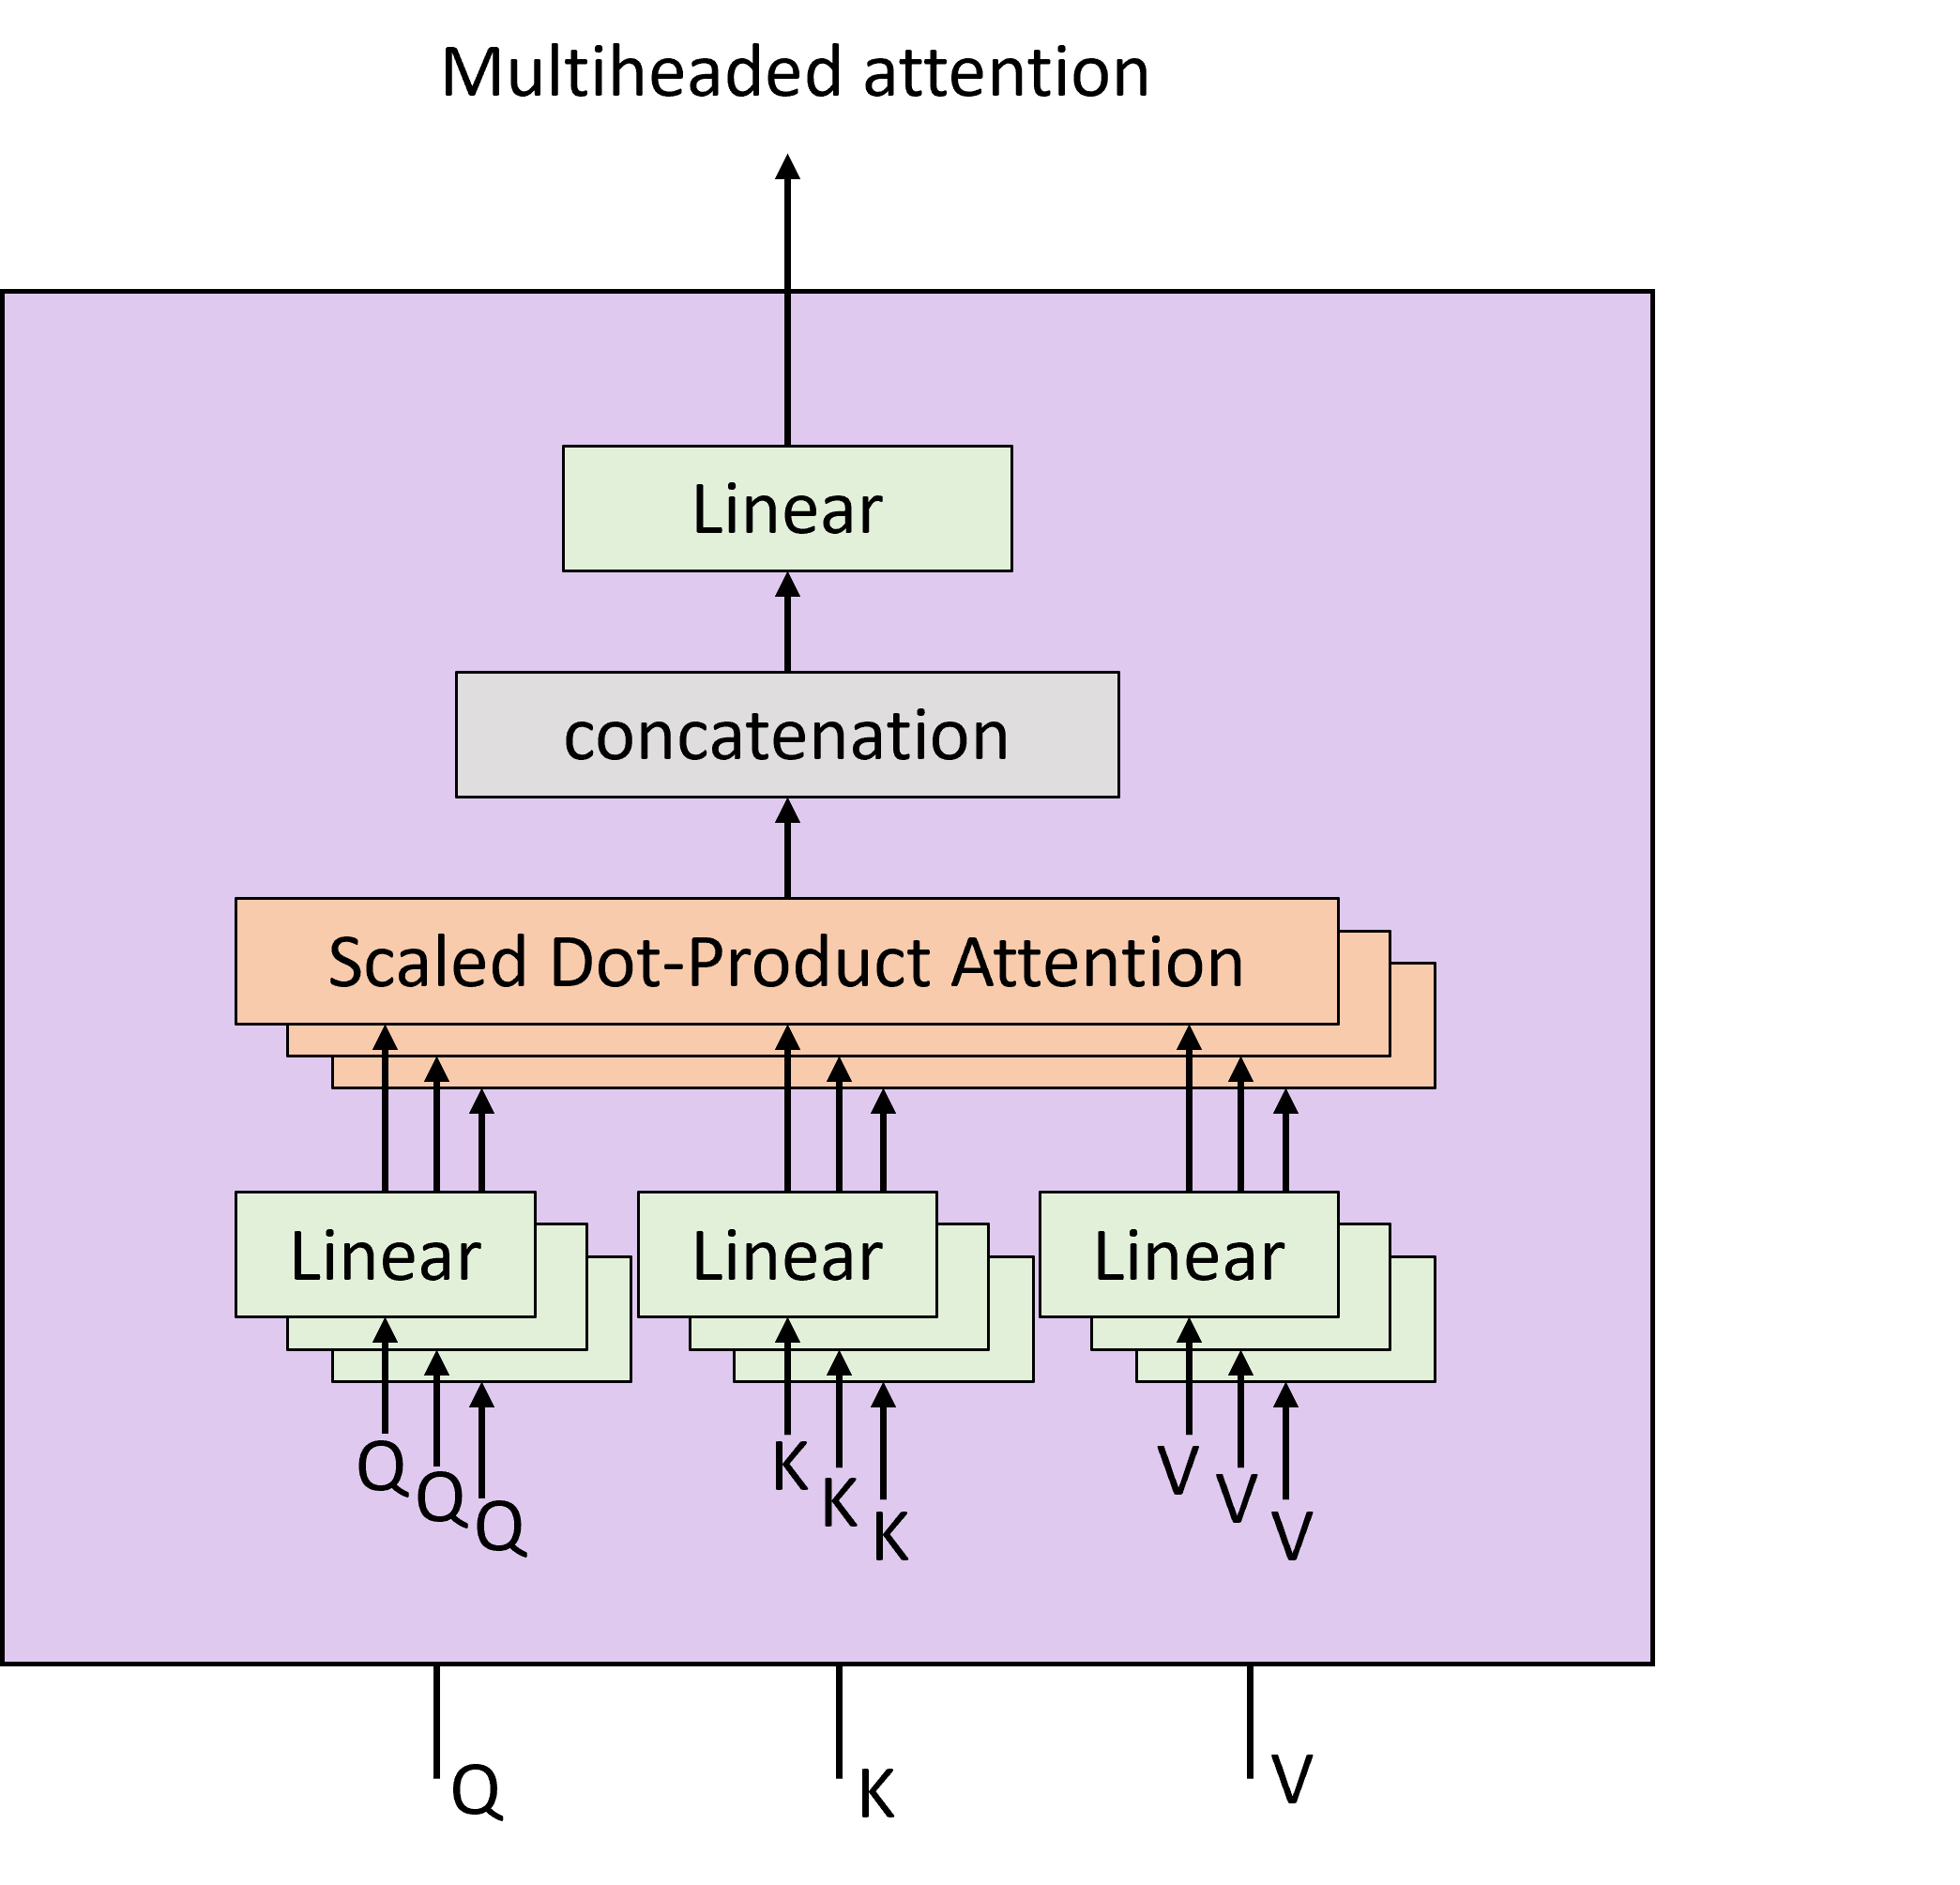
\includegraphics[width=6cm]{img/Multi-headed_attention.png}
    \caption{Figure presenting a multiheaded attention mechanism made based on \cite{46201}}
    \label{fig:MHA}
\end{figure}



The linear projections are an essential part of the system, as they are the trainable part of the multi-headed attention mechanism. In the original paper\cite{46201}, it is stated that the separate attention heads, using different linear projections, seemingly exhibit behavior related to the syntactic and semantic structure of language. This behavior is achieved by the trained linear projections.

\section{Recurrent neural networks}
transformer model are typically superior over Recurrent neural networks (RNN) models and convolutional models, given their numerous appearances on the GLUE NLP benchmark leaderboard\cite{wang2018glue}. But RNN's still have a feature where they are superior to transformer models.
The idea of RNNs is that each input word is processed through the model and becomes the new input for the next word, as shown in figure \ref{fig:RNN_figure}.
In other words, the RNN has a linear path length complexity with respect to the input length (as shown previously in table \ref{table:path_length_complexity}). Furthermore, it also has a linear calculation complexity. Calculation complexities with respect to the input length of different neural network types are given in table \ref{table:calculation_complexity}. Where $n$ is the input word count, $d$ is the dimension of the vector representation, $r$ is the range of words used in a restricted transformer network, and $k$ is the kernel size of a convolutional neural network. 

Even though the transformer has a constant path length dependency, as stated in Section \ref{sec:TF} then every word must still be processed by the multi-headed attention mechanism. Every word is therefore processed with respect to every other word. Even if the longest path length is constant, then the calculation complexity becomes quadratic with respect to the input length. 
Therefore, if $n$ is greater than $d$ in table \ref{table:calculation_complexity}, then a recurrent neural network has fewer calculations than a transformer. Recurrent neural networks are therefore better suited for tasks requiring long input sequences, like thesis summarization.

\begin{figure}[h]
    \centering
    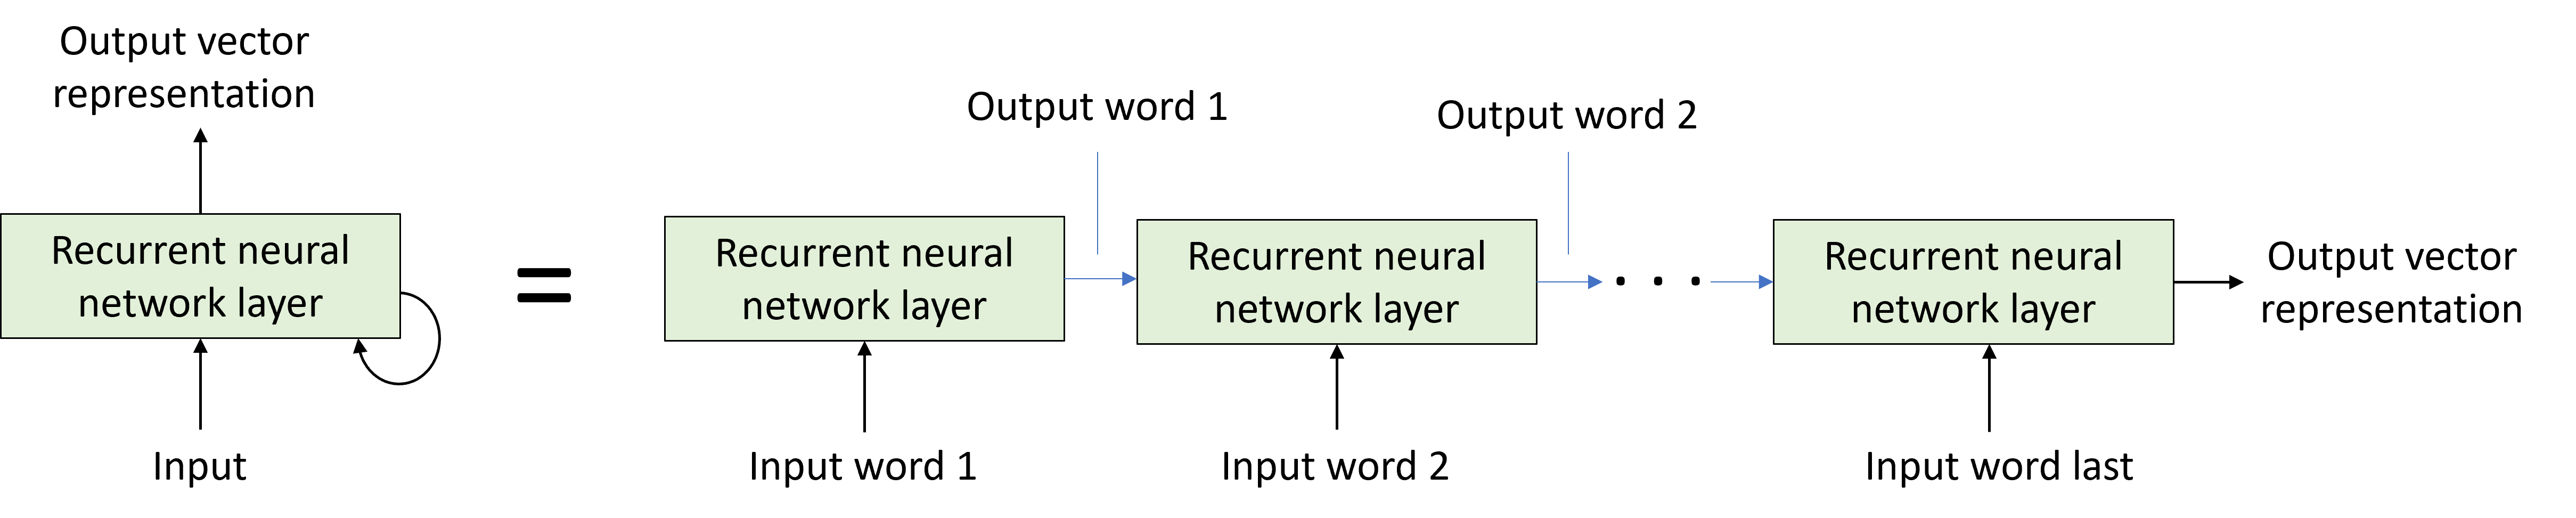
\includegraphics[width=12cm]{img/RNN_model_design.png}
    
    \caption{Figure showing how a recurrent neural network processes data.}
    \label{fig:RNN_figure}
\end{figure}

The RNN encoder model explained in this thesis, is the LSTM model. The next section will go through the encoder models used in this thesis.



\begin{table}[ht]
    \centering
    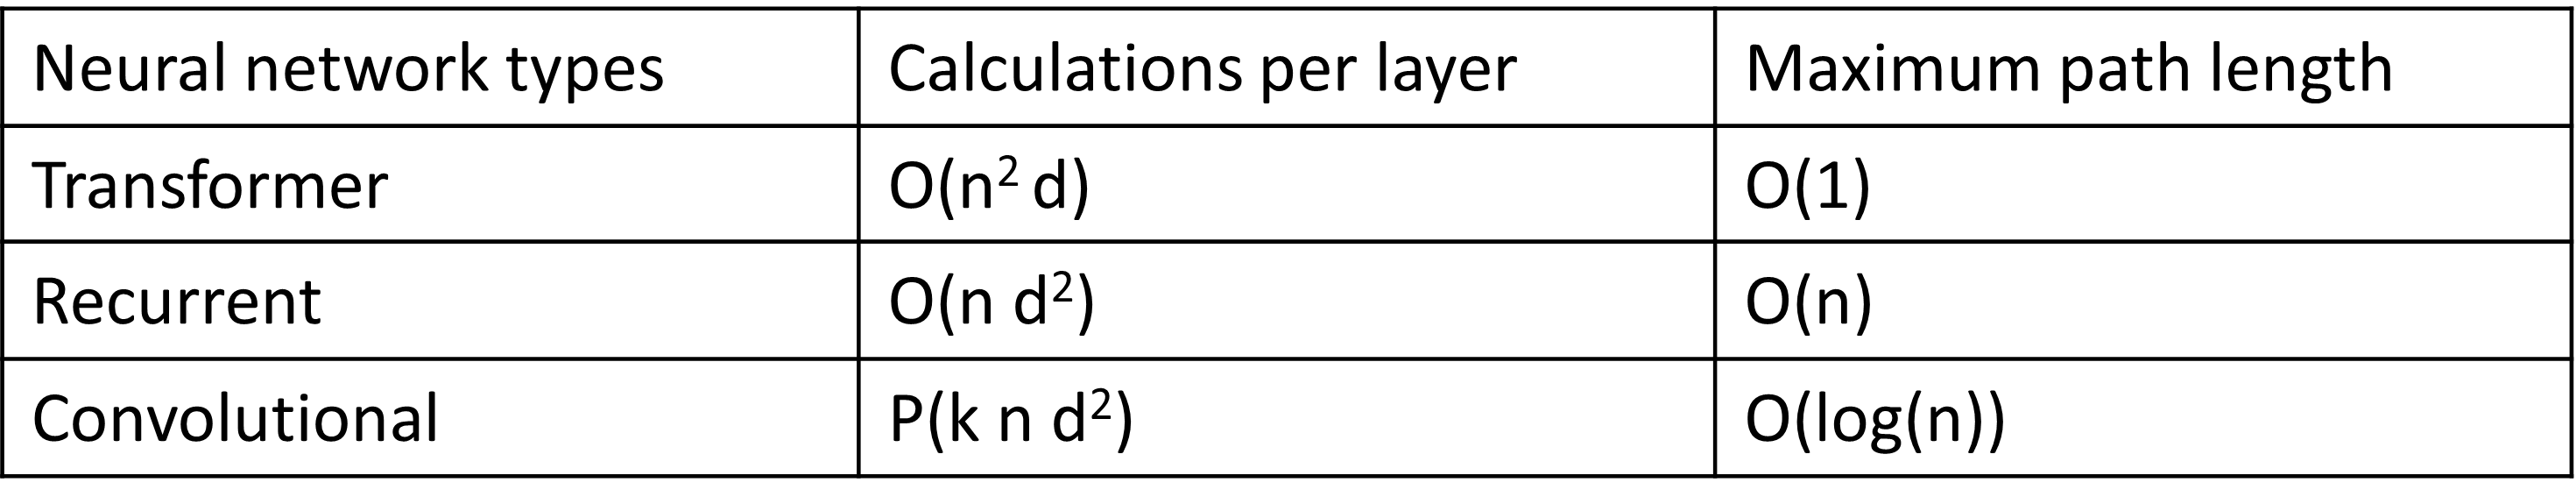
\includegraphics[width=8cm]{img/process_complexity.png}
    \caption{Table showing the processing complexity of different neural networks.}
    \label{table:calculation_complexity}
\end{table}

\section{Encoder models} \label{sec:ED}
There are three main model types for NLP, as shown below.

\begin{itemize}
    \item Encoder-decoder models (sequence-to-sequence)
    \item Encoder models
    \item Decoder models
\end{itemize}

Encoder-decoder models are, in the simplest terms, the full transformer design described in the previous section. The input is processed in the left part of the transformer, and the output is generated in the right part of the transformer. The encoder-decoder model, also called the sequence-to-sequence model, is mostly used for text summarization. The left part of the transformer is the encoder model. It focuses on processing the input, and is usually used for text information extraction, such as assigning grammatical categories or analyzing sentence structure. The right side is called the decoder model. It is used for generating output sentences. This is used for general text-generation tasks.
As this thesis needs a tool that can analyze input sentences and gain information from the input, the encoder model is the most prominent. With encoder models, it can be expected that the model outputs information about the input, rather than more words.

The most common NN encoder model used in this thesis is the BERT model. This model is the encoder model used with the transformers




\subsection{BERT} \label{sec:BERT}
A recent development in the field of neural networks in relation to NLP is the release of the BERT model, which stands for (Bi-directional Encoder Representations Transformer) \cite{47751}. 
BERT, unlike other transformers, is trained using two distinct methods. word-by-word relation and sentence-by-sentence relation. Word-by-word relations are trained by letting the model predict masked words in a sentence, as shown in figure \ref{fig:WBW_training}. Sentence-by-sentence relations are trained by giving the model sentence pairs marked as sentence A and sentence B. The model afterwards determines whether sentence A is the continuation of sentence B in a text. An example is shown in figure \ref{fig:SBS_training}.
 
 
\begin{figure}[ht]
    \centering
    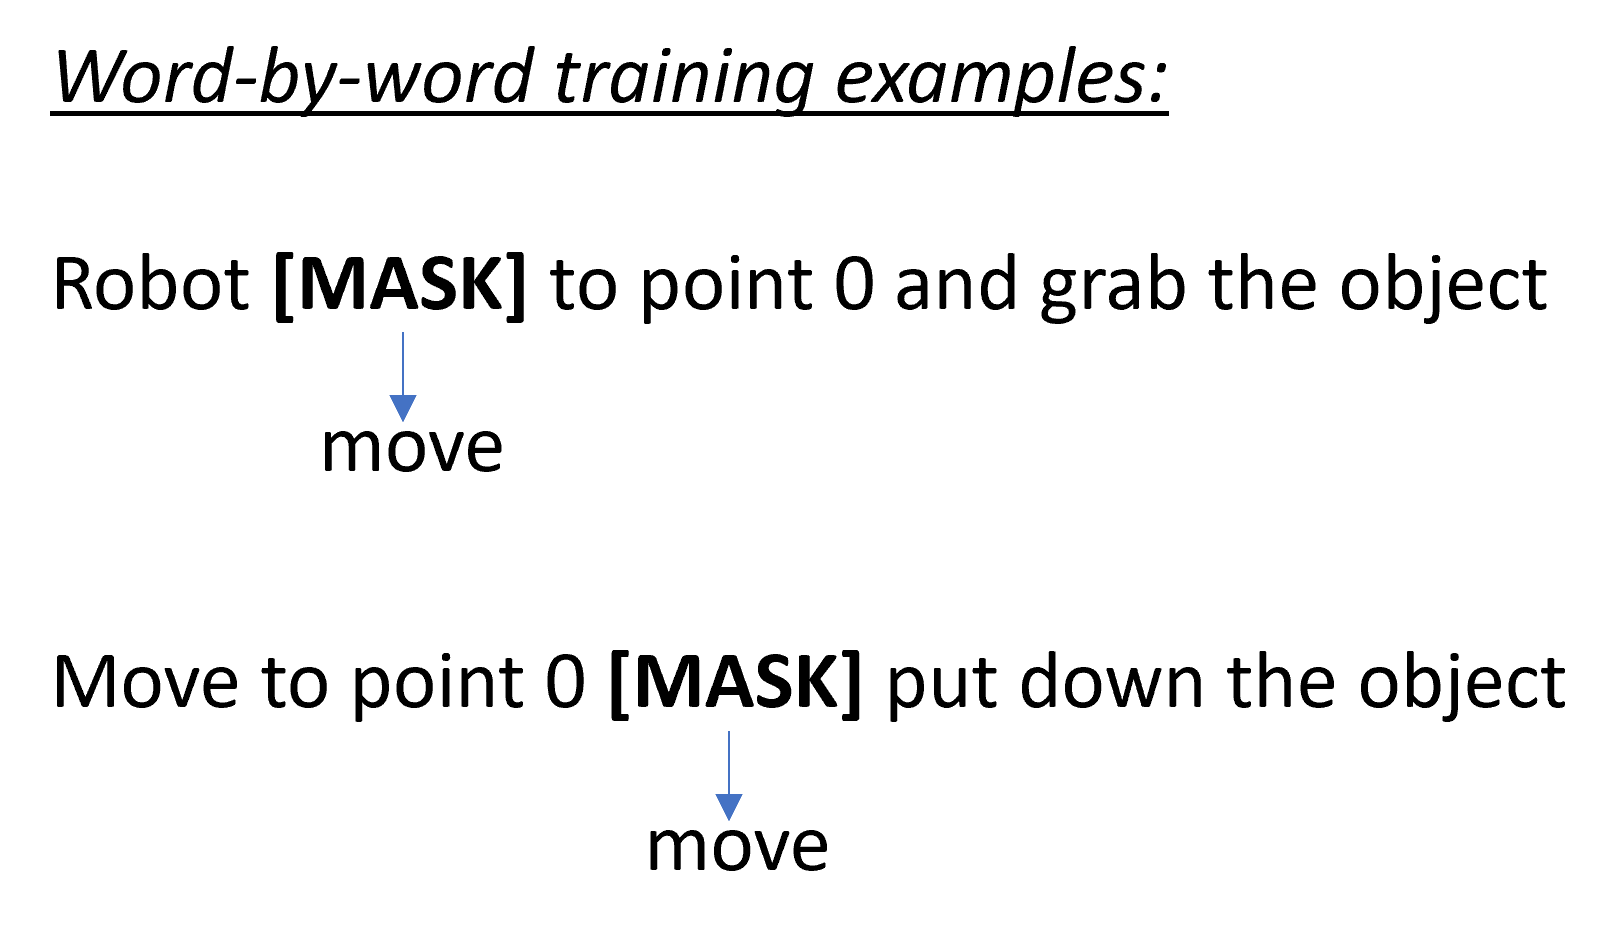
\includegraphics[width=8cm]{img/word-by-word-training.png}
    \caption{Figure shows the training method that learns the model's word-by-word relations.}
    \label{fig:WBW_training}
\end{figure}

\begin{figure}[ht]
    \centering
    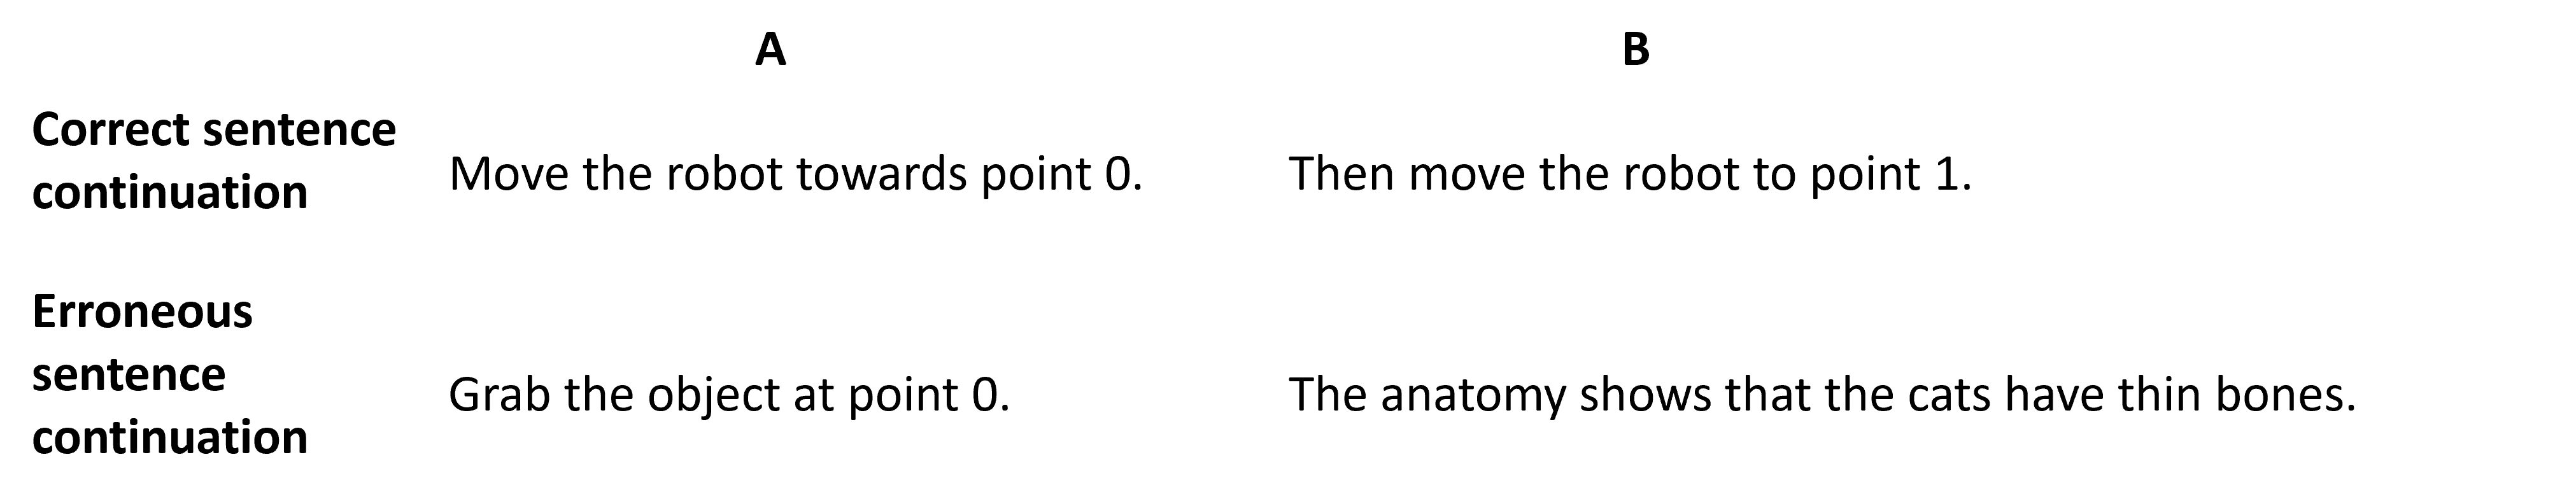
\includegraphics[width=12cm]{img/sentence-by-sentence-relation.png}
    \caption{shows sentence-by-sentence relation training examples, with a correct sentence continuation and a wrong sentence continuation.}
    \label{fig:SBS_training}
\end{figure}



Bi-directionality stems from the BERT model's word-by-word training design, where the full sentences are shown except for the masked word. This is opposed to previous transformer models that were trained left-to-right or right-to-left.
The training methods make the model achieve state-of-the-art results on a wide variety of NLP tasks without task-specific training. In other words, the training allows the BERT model to gain a generalized understanding of natural language. This enables the BERT to be released as a pre-trained language model. All further training will then be done with comprehension of natural language as the starting point. This method is called finetuning and allows the model to train faster on any NLP task. 

The following section describes another important encoder model that is used in this thesis.


\subsection{LSTM} \label{sec:LSTM}
The Long Short Term Memory (LSTM) cell, is a type of RNN node that is widely used for NLP. This model was the prevalent design for NLP tasks before transformers and is still used today. This section will shortly explain how the LSTM models work.
\\\\
RNNs have a linear path dependency. It is therefore also expected, that the representation calculation is done using information from all previous words. But some words are more important to remember than others. This problem makes general RNNs bad at long-term dependencies, as they try to carry information from all previous words into the current word calculation. figure \ref{fig:LSTM_cell} shows a representation of the LSTM cell. 


\begin{figure}[ht]
    \centering
    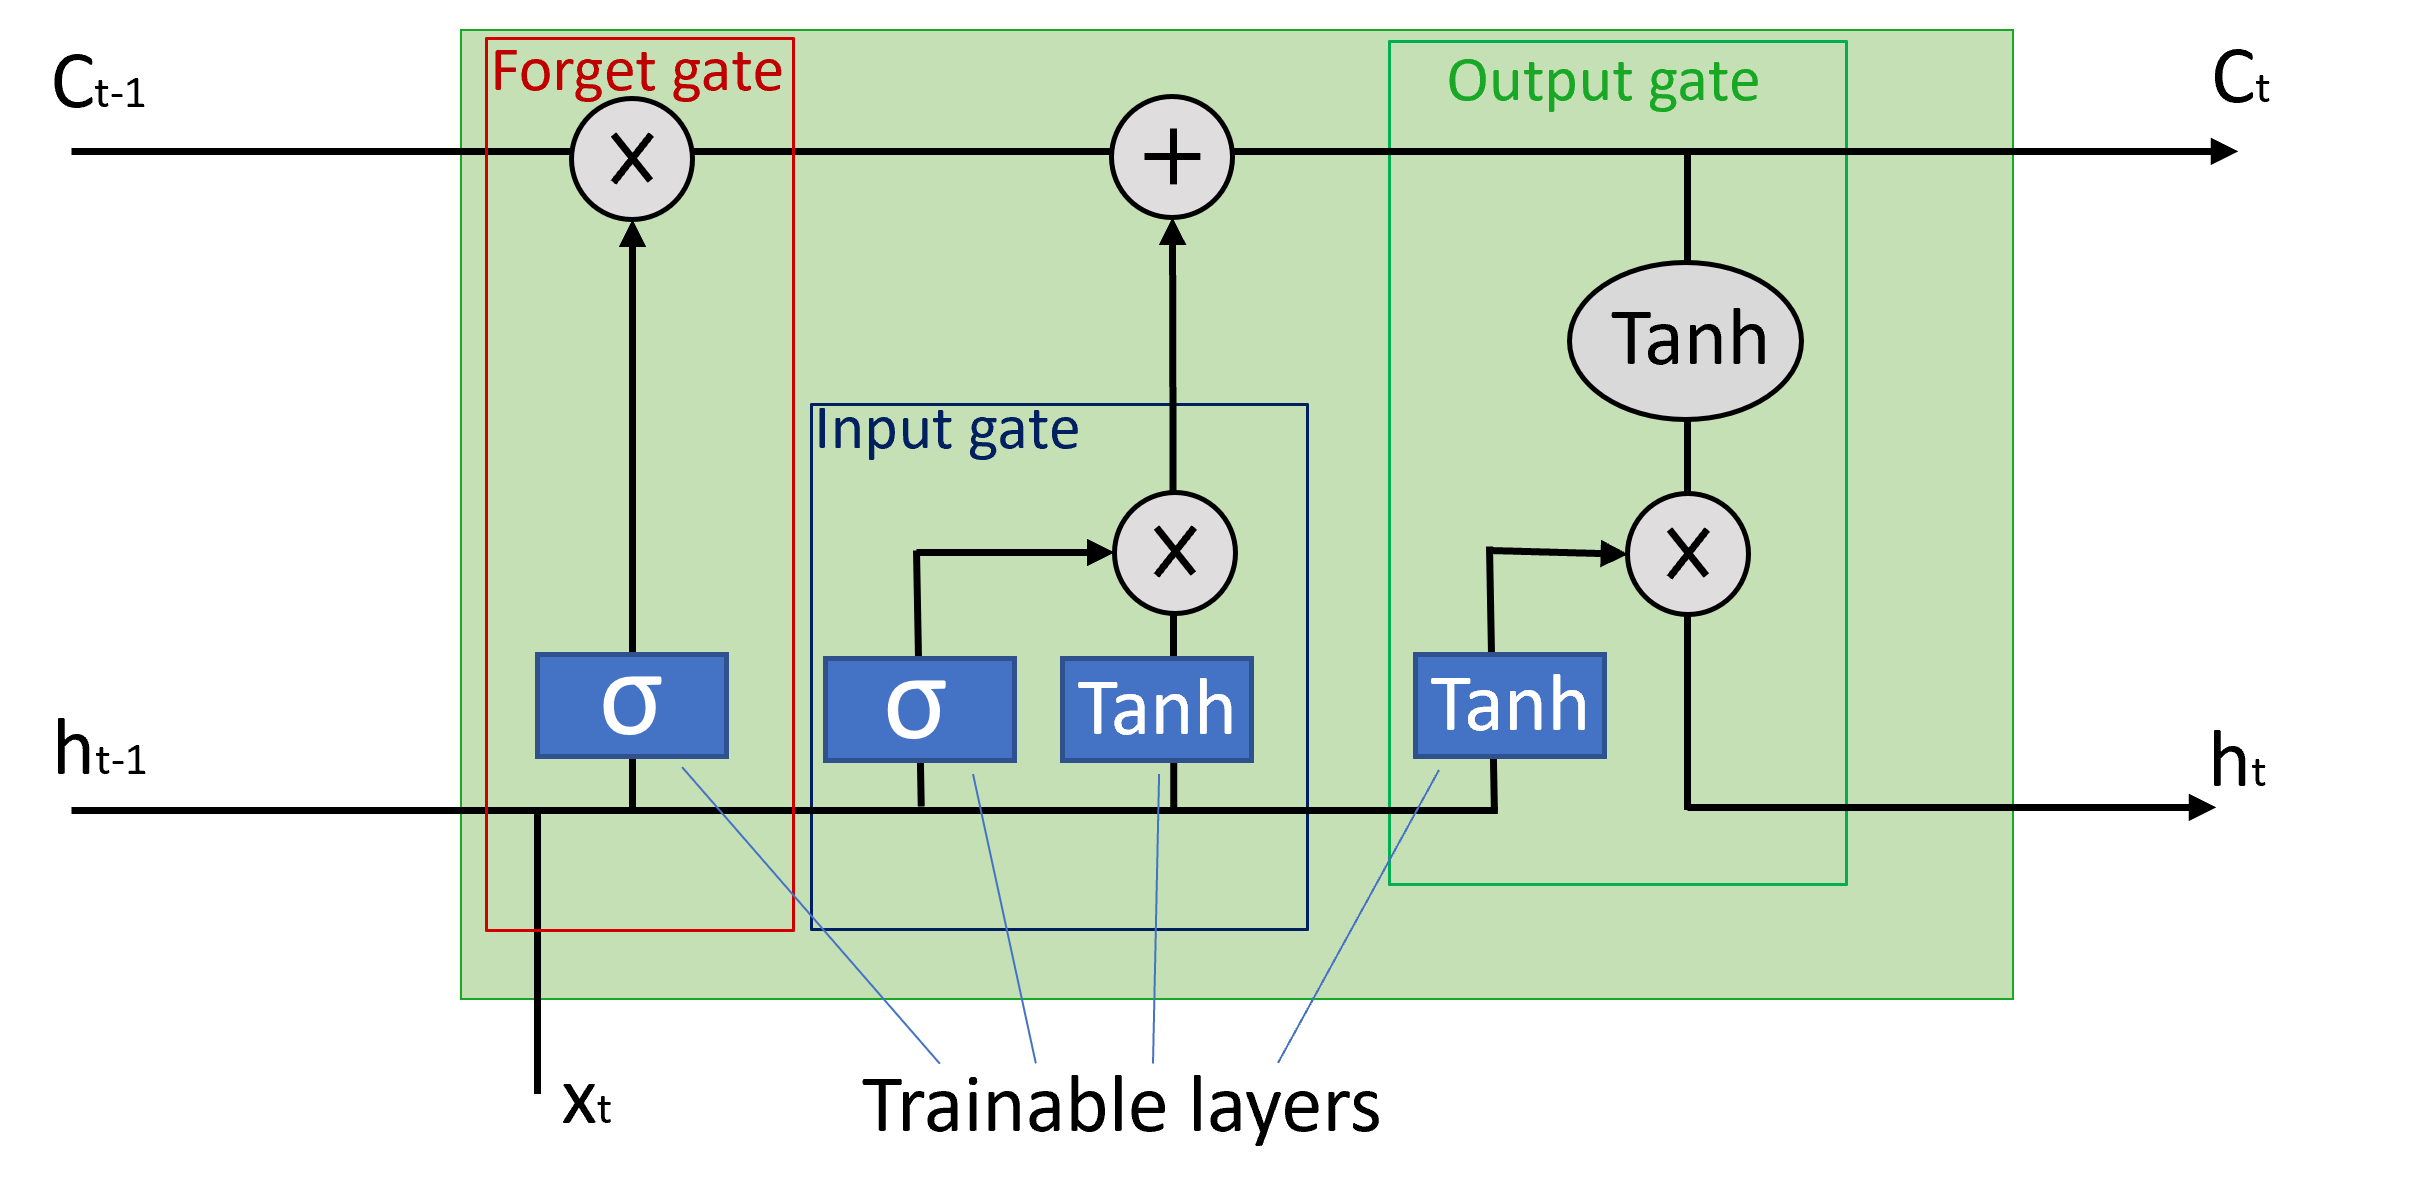
\includegraphics[width=12cm]{img/LSTM_cell.png}
    \caption{Shows a LSTM cell that consists of learnable layers marked with a blue rectangle, and pointwise operations marked as grey circles.}
    \label{fig:LSTM_cell}
\end{figure}

The purpose of the LSTM cell is to train the cell to hold long-term dependencies with higher priorities than meaningless information. The $\text{sigmoid}$ and the $\text{tanh}$ layers marked with a blue rectangle are the trainable layers of the LSTM cell. The sigmoid layer marked in the "Forget gate" is a layer with values ranging from 0 to 1, determining how much input information should be forgotten. Afterward, the sigmoid and the tanh layers in the area named "Input gate" are used to inject information into $C_t$. The last tanh layer within the area named "Output gate" is used to calculate the next hidden state for the next LSTM layer. The use of the LSTM cell is the fundamental block for LSTM models. There are multiple alternative model styles for LSTM models, But they will not be discussed in this thesis.
